% !TeX root = ../main.tex
% Add the above to each chapter to make compiling the PDF easier in some editors.

\chapter{FDSA and SPSA Calibration}\label{chapter:fdsa_and_spsa_calibration}
\section{Literature Review}
The concept of stochastic approximation (SA) was first introduced in 1951 by Robbins and Moro \parencite{spall:2012}. The idea behind SA is to provide a general root-finding method when only noisy measurements of the underlying function are available. Methods for stochastic optimization provide an alternative solution to classical deterministic optimization ones, where nonlinear/high dimensional systems with inherent noise are non-trivial/possible to analyze. There exists different applications for SA methods (business, aerospace engineering, simulation...); for any application, the important part to analyse is how the evaluation of the gradient should be performed, as well as the calculation of the gain sequences \(a_k\) and \(c_k\) of the algorithm. The general approach in SA is give as the form:

\begin{equation}
\boldsymbol{\hat{\theta}_{k+1}} = \boldsymbol{\hat{\theta}_k} - a_k\boldsymbol{\hat{g}}_k(\boldsymbol{\hat{\theta}_k})
\label{eq:1}
\end{equation}

where \(\boldsymbol{\hat{g}}_k(\boldsymbol{\hat{\theta}_k})\) is an estimate of the gradient at the value \(\boldsymbol{\hat{\theta}_k}\) and \(\boldsymbol{\theta}\) is a vector variable. The main goal of the optimization approach is to find a vector \(\boldsymbol{\theta}\) that minimizes a scalar-valued loss (objective) function. In this report, 2 different approaches to SA algorithms will be discussed. These are FDSA and SPSA including some variations of the later. 

\subsection{FDSA}
Finite-Difference Stochastic Approximation (FDSA) is a gradient approximation method used in scenarios where the true gradient evaluation can not be calculated. FDSA is gradient free, which means that for the problem and functions involved, the partial derivatives are somehow expensive to compute. Gradient free methods proceed without going through the process of calculating the first or second derivatives, hence the name "gradient free". For a two-sided FDSA, we may use the following form together with \ref{eq:1}:

\begin{figure}[htpb]
  \centering
  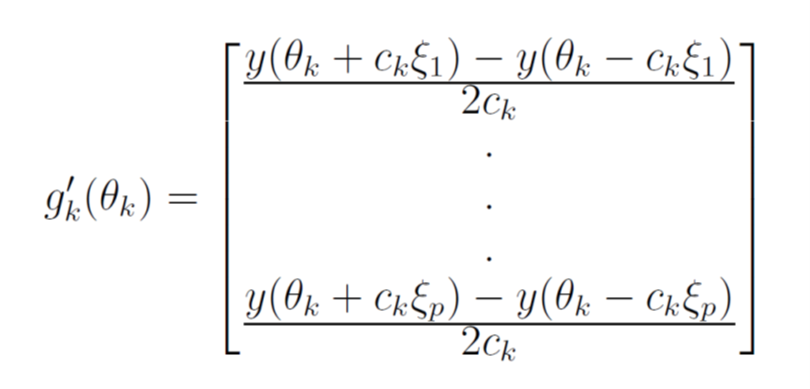
\includegraphics[width=0.5\textwidth]{figures/equation_2_sided_fdsa.png}
  \label{fig:eq2}
\end{figure}

where \(\xi_i\) represents a vector with a one at the position i and zero elsewhere and the gain sequence \(c_k > 0\) is the perturbation/difference magnitude. While using this method, the gradient is evaluated on the noisy measurements calculated after perturbing a single variable sequentially. This is important to mention, as for a p-dimensional problem it requires \(2*p + 1\) loss (objective) function evaluations for every single gradient approximation. As the dimension p of the problem grows large, the number of objective function evaluations required may become prohibitive. This means, for a large enough high-dimensional problem, FDSA may be infeasible to use. 

\subsection{SPSA}
Simultaneous Perturbation Stochastic Approximation (SPSA) is another gradient (free) approximation method introduced by Spall in 1998 \parencite{spall:1998} as a different approach for gradient evaluation. The most remarkable contribution of this approach compared to FDSA, lies on the number of loss function evaluations per iteration in order to evaluate the gradient: only 2 evaluations required, regardless of the size of p. In this approach, the vector \(\boldsymbol{\hat{\theta}_k}\) is perturbed simultaneously by means of a random perturbation vector \(\boldsymbol{\Delta_k}\) which has a given distribution specified by the user. Replacing \(\xi_i\) in equation \ref{eq:1} by \(\boldsymbol{\Delta_k}\), we can derive the following form:

\begin{figure}[htpb]
  \centering
  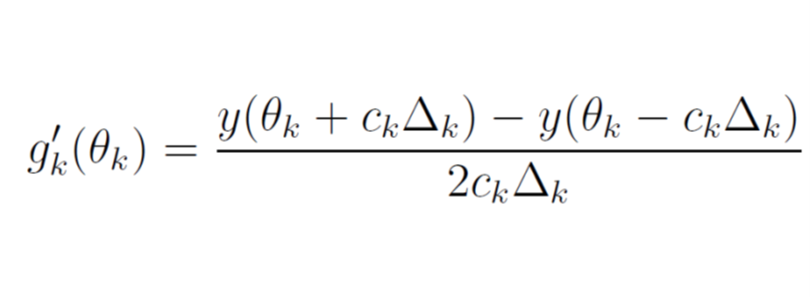
\includegraphics[width=0.5\textwidth]{figures/equation_2_sided_spsa.png}
  \label{fig:eq3}
\end{figure}

While FDSA requires \(2*p\) loss function evaluations due to the sequential perturbation of the vector \(\boldsymbol{\hat{\theta}}\), SPSA only requires \(1/p\) times the number of function evaluations of FDSA as it can be appreciated in the previous equation \parencite{spall:2012}. This yields to p-fold savings per iteration of the objective function calculation, which provides SPSA the possibility to scale accordingly regardless the size p of the problem, in contrast to FDSA which is unlikely to scale for a large enough high-dimensional problem. 

\subsection{PC-SPSA}
PC-SPSA is a combination of the SPSA algorithm and the statistical procedure principal component analysis (PCA) introduced in \parencite{pcspsa:2018}. In this approach, a dimension reduction technique is applied in order to calculate the variance of prior estimates in the form of PC component directions. By doing so, the PC component directions are then used to evaluate PC scores which are then calibrated by means of SPSA. In general, the problem size is reduced from a high dimensional OD matrix, to a couple of PC scores for demand calibration. This new approach provides two major advantages over traditional SPSA. The first one is the dimensionality reduction as it has been previously explained: instead of taking into account a complete OD matrix for calibration, the variability of the entire data set can be capture in the principal components, which in turn increases the performance of SPSA considerably. Secondly, the number of variables to estimate is reduced considerably as well. 

\section{Non-linear synthetic function calibration}
Before starting to calibrate a simulated traffic network, such a Sioux Falls or Munich, a non-linear synthetic function has been used for calibration purposes. The main goal of the synthetic function is to replace the dynamic traffic simulator (in this case SUMO) and observe how FDSA and SPSA perform on different synthetic scenarios. This process has been helpful to understand how the different calibration parameters affect the calibration output as well as the \textbf{performance} and \textbf{accuracy} of FDSA and SPSA on large and small dimensional problems.

\subsection{Function selection: Quadratic vs Rastrigin vs Drop-Wave}

To this end, three different functions have been tested under the same calibration parameters. The first function tested was a regular quadratic function. In order to provide a more interesting synthetic calibration scenario, the functions Rastrigin and Drop-Wave have been used \parencite{OTF}. Both functions are well know test functions in the context of simulation experiments and optimization problems. Both functions pose a high complexity problem with several local minima, for this reason both functions have been chosen as alternative to the more standard quadratic function in order to evaluate the \textbf{performance} and \textbf{accuracy} of the algorithms in question. 

\subsection{Rastrigin and Drop-Wave functions}
In one hand, the Rastrigin function provides several local minima, it is highly multimodal and locations of the minima are regularly distributed. The form of the Rastrigin function has the following form:

\begin{figure}[htpb]
  \centering
  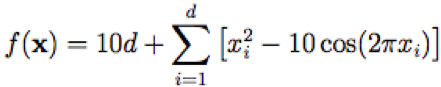
\includegraphics[width=0.4\textwidth]{figures/rastrigin-function.png}
  \label{fig:eq4}
\end{figure}

This function poses over d dimensions, it is normally evaluated evaluated on the hypercube xi from -5.12 to 5.12 and has a global minimum at \(\boldsymbol{f(x*)} = 0\) at \(x* = (0, ..., 0)\). A 3 dimensional representation of the function is shown in figure \ref{eq5-fig}a. 
\vskip 0.2in
In the other hand, the Drop-Wave function is multimodal, highly complex and locations of the minima are not regularly distributed. The form of the Drop-Wave function has the following form:

\begin{figure}[htpb]
  \centering
  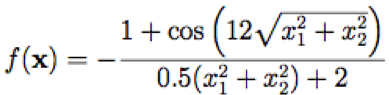
\includegraphics[width=0.35\textwidth]{figures/drop-wave-function.png}
  \label{fig:eq5}
\end{figure}

This function poses over 2 dimensions, it is normally evaluated on the square xi from -5.12 to 5.12 and has a global minimum at \(\boldsymbol{f(x*)} = -1\) at \(x* = (0, 0)\). A 3 dimensional representation of the function is shown in figure \ref{eq5-fig}b.

\begin{figure}[htpb]
  \centering
    \subfloat[3D representation of the Rastrigin function]{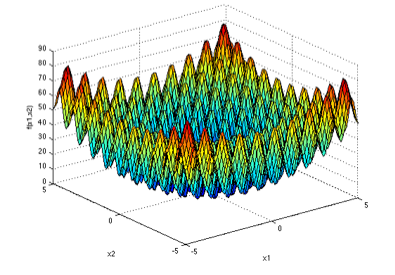
\includegraphics[width=0.5\columnwidth]{figures/rastrigin-2d.png}}
    \qquad
    \subfloat[3D representation of the Drop-Wave function]{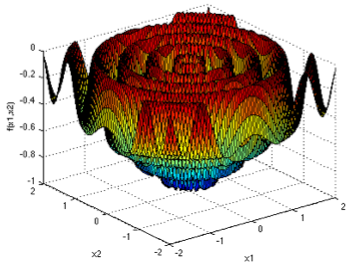
\includegraphics[width=0.5\columnwidth]{figures/drop-wave-2d.png}}
  \caption{Synthetic Functions}
  \label{eq5-fig}
\end{figure}

\subsection{Function calibration: Quadratic vs Rastrigin vs Drop-Wave}
For the function calibration approach, the calibration parameters on table \ref{tab:calibration-params} where chosen for both, FDSA and SPSA. These calibration parameters include the necessary information to compute the gain sequences \(a_k\) and \(c_k\) of the algorithm, the gradient and perturbation vector. 
\vskip 0.2in
\vskip 0.2in
\vskip 0.2in
\vskip 0.2in
\vskip 0.2in
\vskip 0.2in

\begin{table}[htpb]
  \centering
  \begin{tabular}{l l l l l l l l l l}
    \toprule
      - & a & c & A & Alpha & Gamma & h & G & N & seg\\
    \midrule
      SPSA & 300 & 1 & 10 & .702 & .151 & .7 & 3 & 200 & 5 \\
      FDSA & 300 & 1 & 10 & .702 & .151 & .7 & - & 200 & 5 \\
    \bottomrule
  \end{tabular}
  \caption[Calibration Parameters]{Calibration parameters for synthetic function calibration}
  \label{tab:calibration-params}
\end{table}

Using these calibration parameters, the following results have been obtained:

\begin{table}[htpb]
  \centering
  \begin{tabular}{l l l l}
    \toprule
      Function & Algorithm & Time (s) & Best RMSN \\
    \midrule
      Quadratic & SPSA & .464 & .315  \\
      Quadratic & FDSA & 18.52 & .0025  \\
      Rastrigin & SPSA & 1.096 & .0187  \\
      Rastrigin & FDSA & 86.65 & .0015  \\
      Drop-Wave & SPSA & .576 & .100  \\
      Drop-Wave & FDSA & 32.41 & .0019  \\
    \bottomrule
  \end{tabular}
  \caption[Calibration Results]{Calibration results for synthetic function calibration selection}
  \label{tab:calibration-results}
\end{table}

As it can be appreciated in the results in table \ref{tab:calibration-results} and figure \ref{fig:spsavsfdsa-comparison}, the most notorious difference between FDSA and SPSA is the time the algorithms require to compute 200 iterations to calibrate the synthetic function chosen (smaller RMSN). The RMSN value represents the goodness of fit for the calibration process. This measurement is widely used when it comes to model calibration and model accuracy testing (observation vs prediction accuracy). The smaller RMSN obtained, the better accuracy the model posses. 
\vskip 0.2in
While FDSA provides a more accurate/smaller value for the RMSN of the calibration after a couple of iterations, the time to compute that value is considerably higher in comparison to SPSA. As it has been mentioned in the literature review section, for a high enough dimensional problem, FDSA is more likely not to work due to the computational overhead required by the algorithm. Furthermore, the p-fold objective function calculation savings per SPSA iteration reflect directly on the performance of the algorithm. 
\vskip 0.2in
Based on the results obtained from the comparison between both algorithms and the three synthetic functions, the Drop-Wave function has been chosen for further analysis. The reason for this selection is because the results for both algorithms, FDSA and SPSA, lie in between of the ones obtained for the Rastrigin and Quadratic functions. Having performed this analysis, 4 different synthetic study cases have been calibrated using the non-linear Drop-Wave function.

\begin{figure}[htpb]
  \centering
    \subfloat[SPSA vs FDSA on Quadratic function]{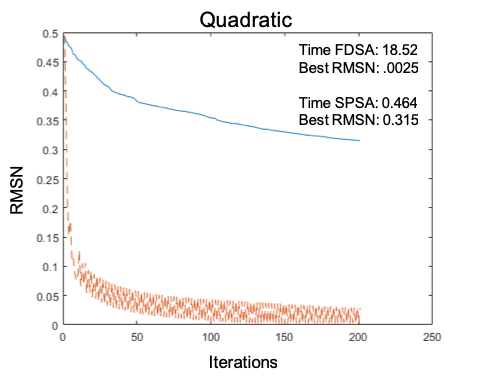
\includegraphics[width=0.5\columnwidth]{figures/quadratic-spsa-fdsa.png}}
    \subfloat[SPSA vs FDSA on Rastrigin function]{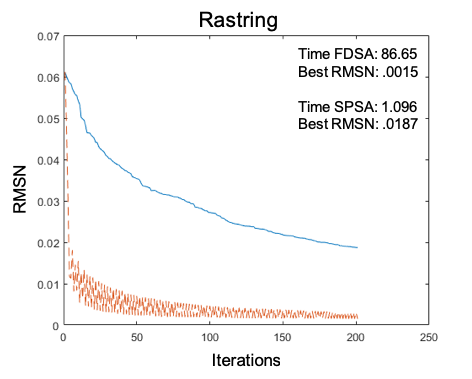
\includegraphics[width=0.5\columnwidth]{figures/rastring-spsa-fdsa.png}}
    \qquad
    \subfloat[SPSA vs FDSA on Drop-Wave function]{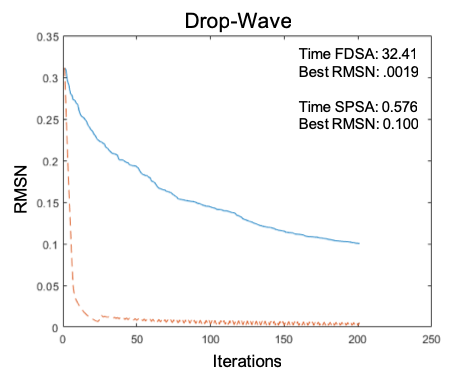
\includegraphics[width=0.7\columnwidth]{figures/drop-wave-spsa-fdsa.png}}
  \caption{Synthetic Functions}
  \label{fig:spsavsfdsa-comparison}
\end{figure}

\subsection{Case study calibration using Drop-Wave as synthetic function}
For the synthetic study case calibration, the study cases in table \ref{tab:demand-scenarions} have been defined beforehand.

\begin{table}[htpb]
  \centering
  \begin{tabular}{l l l l l l}
    \toprule
      Case & Reduction coeff. & Randomization coeff. & Zones & Counts & Iterations \\
    \midrule
      A & .7 & .3 & 10 & .2 & 200  \\
      B & .7 & .3 & 40 & .2 & 200  \\
      C & .7 & .3 & 30 & .4 & 200  \\
      D & .7 & .3 & 30 & .7 & 200  \\
      E & .7 & .3 & 40 & .7 & 10000  \\
    \bottomrule
  \end{tabular}
  \caption[Calibration Study Cases]{Study cases for demand calibration}
  \label{tab:demand-scenarions}
\end{table}

For comparison purposes, case B and E will be used. As it can be observed in figure \ref{fig:demand-study-cases}b, FDSA took around 24 minutes to compute 200 iterations of the algorithm reaching a RMSN of .0032. On the other hand, FDSA took 3.5 seconds and reached a RMSN of .21. Case study E has been added as a variation for case B for a more detailed analysis between the \textbf{performance} and \textbf{accuracy} of FDSA and SPSA. For this analysis, both algorithms will stop the calibration procedure when reaching a given convergence criteria smaller than .1 for the RMSN. The idea here is to compare the number of iterations against the time required to reach the convergence criteria and observe the accuracy obtained under this conditions. Observing figure \ref{fig:demand-study-case-e}, FDSA took 5 iterations to reach the convergence criteria for the RMSN, whereas SPSA took around 360 iterations to do so. However, the performance of FDSA was almost 6 times slower (in regards of time) in comparison to SPSA.

\begin{figure}[htpb]
  \centering
  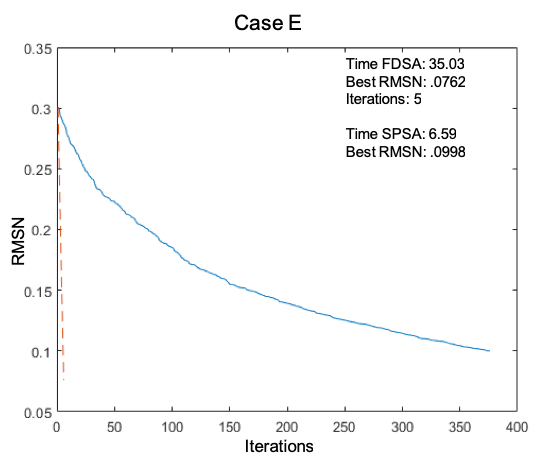
\includegraphics[width=0.5\textwidth]{figures/demand-case-e.png}
  \caption{Demand scenario E}
  \label{fig:demand-study-case-e}
\end{figure}

\begin{figure}[htpb]
  \centering
    \subfloat[Results for scenario A]{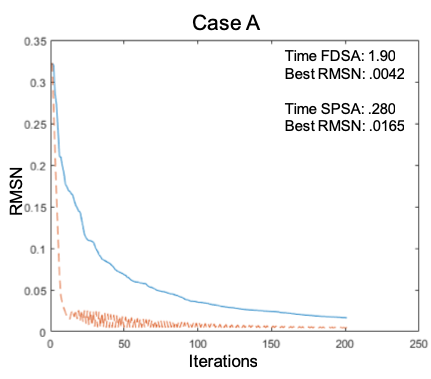
\includegraphics[width=0.5\columnwidth]{figures/demand-case-a.png}}
    \subfloat[Results for scenario B]{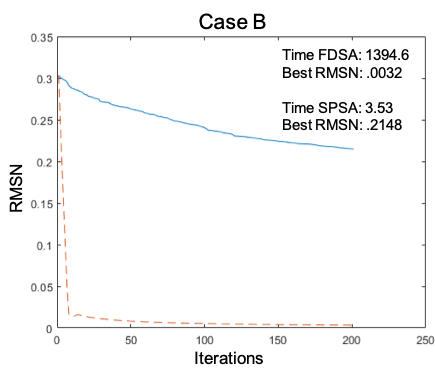
\includegraphics[width=0.5\columnwidth]{figures/demand-case-b.png}}
    \qquad
    \subfloat[Results for scenario C]{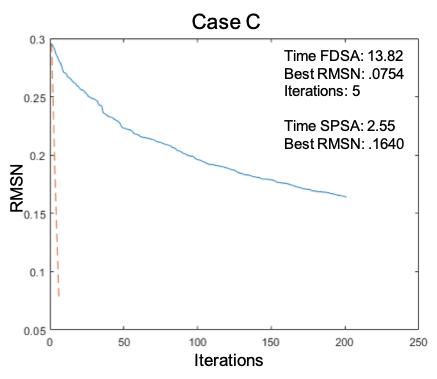
\includegraphics[width=0.5\columnwidth]{figures/demand-case-c.png}}
    \subfloat[Results for scenario D]{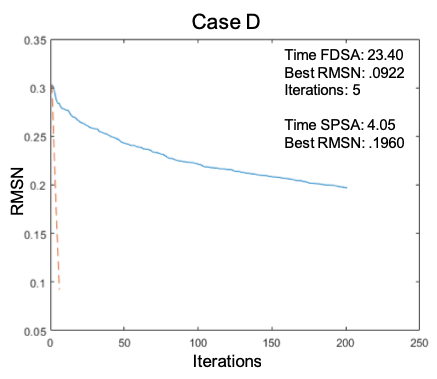
\includegraphics[width=0.5\columnwidth]{figures/demand-case-d.png}}
  \caption{Demand Study Cases}
  \label{fig:demand-study-cases}
\end{figure}

\section{Sensitivity analysis}
\subsection{OD Zones, reduction and randomization coefficients}
For the sensitivity analysis calculation, different demand scenarios where calibrated. In order to do so, a programmatic implementation in Matlab has been used. In this implementation, 3 scenario parameters have been iterated for the scenario creation: number of OD zones from 10 to 50 with a step size of 10, reduction coefficient from .1 to .9 with a step size of .1 and randomization coefficient from .1 to .5 with a step size of .1. The code implementation can be seen in the following code listing.

\lstinputlisting{figures/sensitivityAnalysis.m}

For each scenario result obtained after the calibration process using SPSA, a .mat file has been stored for further analysis. From a total of 225 calibrations, the top 5 results per OD zone and the top 5 for 30 OD zones have been selected for further analysis and can be observed in figure \ref{fig:top-5-sensitivity}.

\begin{figure}[htpb]
  \centering
    \subfloat[Top 5 results, 1 per OD Zone]{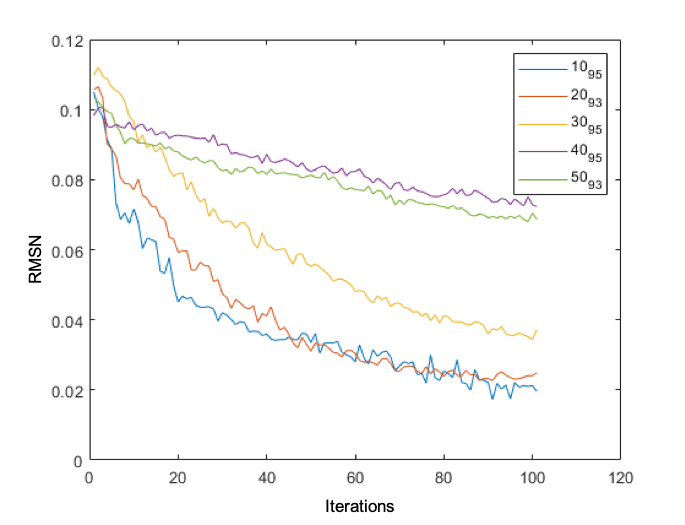
\includegraphics[width=0.5\columnwidth]{figures/top-5-sensitivity.png}}
    \subfloat[Top 5 results, 30 OD Zones]{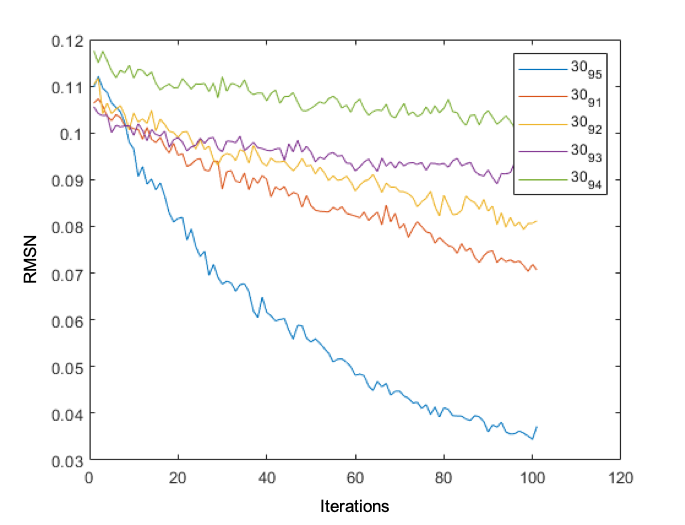
\includegraphics[width=0.5\columnwidth]{figures/top-5-sensitivity-30.png}}
  \caption{Top 5 results for sensitivity analysis}
  \label{fig:top-5-sensitivity}
\end{figure}

Something interesting to notice about the results obtained is that by increasing the reduction coefficient, the RMSN of the calibration improved. In figure \ref{fig:top-5-sensitivity}a all the top results per OD zone fall in the range where the reduction coefficient for the scenario creation was set to the highest value, which is .9. In figure \ref{fig:top-5-sensitivity}b also the top 5 results where found where the reduction coefficient for the scenario creation was set to the highest value. As for the randomization coefficient, it does not seem to provide a clear meaning with respect to the results obtained. In order to provide a different perspective with respect to the reduction coefficient and its impact in the RMSN obtained from the calibration process, figure \ref{fig:top-sensitivity} shows a different schematic which contains different results for the same number of OD zones, but different reduction coefficient values.  

\begin{figure}[htpb]
  \centering
  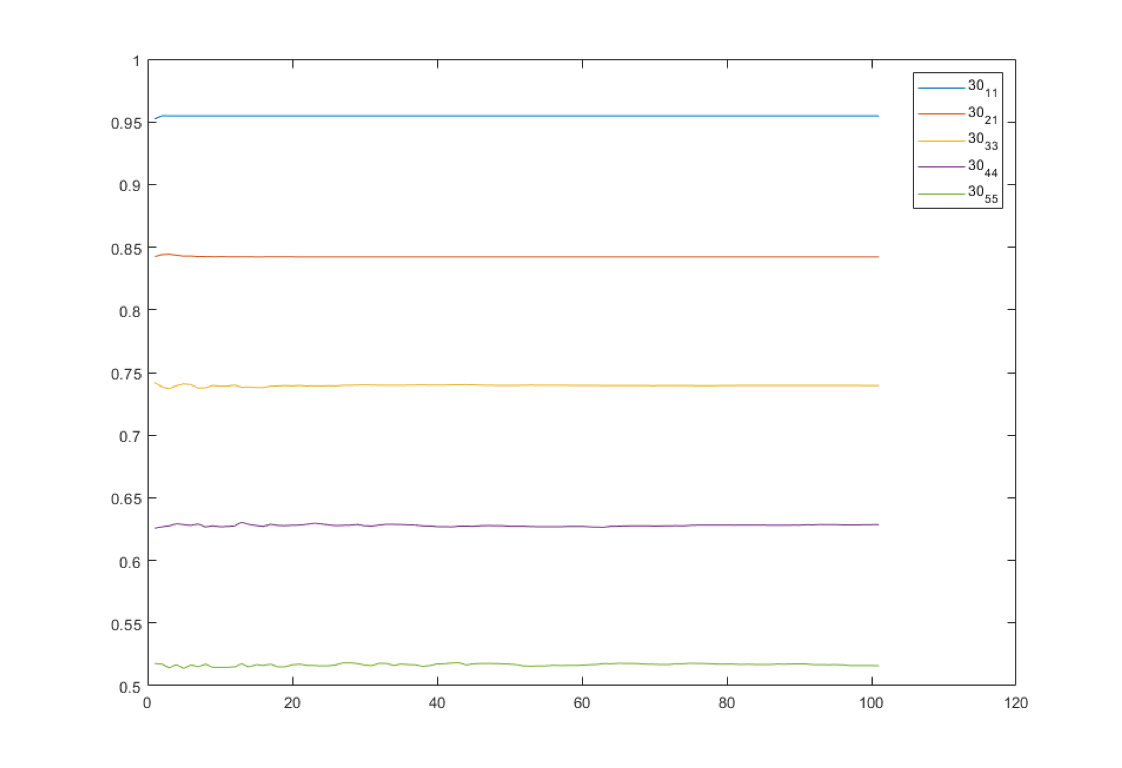
\includegraphics[width=0.8\textwidth]{figures/top-sensitivity.png}
  \caption{Results comparison using same OD zones, but different coefficients}
  \label{fig:top-sensitivity}
\end{figure}

The purpose of this comparison is to show how the reduction coefficient affects the output of the calibration. For a higher the reduction coefficient, the RMSN starts at a smaller value. 

\section{Comparison FDSA and SPSA - final remarks}
As discussed in the previous section both algorithms are capable of reaching acceptable convergence values. Despite of this, for a bigger calibration problem, SPSA would be a better choice compared to FDSA. For a rather small problem, FDSA can provide more accurate results than SPSA and within a reasonable amount of time. Both algorithms could be equally accurate, it all resides on how the calibration parameters for the calibration are chosen. However, for a large enough problem, FDSA is most likely unable to converge to a significant value.  